\documentclass{article}

\usepackage[utf8]{inputenc}
\usepackage[brazil]{babel}

\usepackage{bera}
\usepackage{pdflscape}
\usepackage{gantt} % http://www.martin-kumm.de/tex_gantt_package.php

\usepackage{colortbl}
\usepackage{xspace}
\usepackage{url}


\newcommand\blfootnote[1]{%
  \begingroup
  \renewcommand\thefootnote{}\footnote{#1}%
  \addtocounter{footnote}{-1}%
  \endgroup
}


\usepackage{listingsutf8}
\lstdefinelanguage{pseudocode}
 {morekeywords={se,senao,enquanto,repita,ate,para,retorne},
  %keywordstyle=\fontfamily{fvm}\fontseries{b}\fontshape{b}\selectfont,
  keywordstyle=\fontfamily{fvs}\fontseries{b}\selectfont\bfseries,
  basicstyle=\footnotesize\fontfamily{fvs}\fontshape{n}\selectfont,% \footnotesize was before \fontfamily
  commentstyle=\fontfamily{fvs}\selectfont\slshape,%
  morecomment=[l][commentstyle]{//},
  morecomment=[s][commentstyle]{{/*}{*/}},
  sensitive=false,%
  inputencoding=utf8,
literate={á}{{\'a}}1
         {Á}{{\'A}}1
         {é}{{\'e}}1
         {í}{{\'i}}1
         {Í}{{\'I}}1
         {ó}{{\'o}}1
         {ú}{{\'u}}1
         {à}{{\'a}}1
         {À}{{\`a}}1
         {ã}{{\~a}}1
         {â}{{\^a}}1
         {ê}{{\^e}}1
         {õ}{{\~o}}1
         {ô}{{\^o}}1
         {ç}{{\c{c}}}1,
  string=[d]"
}[keywords,comments,strings]

\lstset{%
%backgroundcolor=\color{Gray},% /usr/share/texmf-texlive/tex/generic/dvips/colordvi.sty
showstringspaces=false,%
%%basicstyle=\fontfamily{cmtt}\fontshape{n}\selectfont,% \footnotesize was before \fontfamily
%%commentstyle=\fontfamily{cmtt}\fontshape{it}\selectfont,%
frame=none,%single,%
texcl=true,%
%extendedchars=\true,
inputencoding=utf8,
language=pseudocode
}
\makeatletter
\define@key{MyCode}{width}[\linewidth]{\def\width{#1}}
\define@key{MyCode}{title}[]{\def\algotitle{#1}}
\define@choicekey*+{MyCode}{type}[\val\nr]{proc,func,algo,none}[none]{%
\ifcase\nr\relax
\def\type{Procedimento}
\or
\def\type{Função}
\or
\def\type{Algoritmo}
\or
{}
\fi
}{\@latex@error{Erroneous value for a choice key}
  {Invalid value '#1' for key 'type' of family Mycode}%
}
\define@key{MyCode}{lstoptions}[]{\def\lstoptions{#1}}
\presetkeys{MyCode}{width,type,lstoptions}{}
\makeatother

\lstnewenvironment{pseudo}[1][]%
{  \setkeys{MyCode}{#1}
   \noindent
   \minipage[t]{\width}
   \vspace{0cm}
   %\noindent\rule[0.4ex]{\linewidth}{1pt}
   \hrule
   \ifdefined\algotitle
     \vspace{0.2\baselineskip}
     \ifdefined\type\relax
           {\bfseries \type}
     \fi
     \algotitle
     \vspace{0.2\baselineskip}
     \hrule
   \fi
   \vspace{0.2\baselineskip}
   \lstset{language=pseudocode,frame=none,mathescape=true,\lstoptions}}
{\hrule\vspace{0.5\baselineskip} %\noindent\rule[0.1ex]{\linewidth}{1pt}
 \vfill\endminipage}


\usepackage{pgf,tikz}
\usepackage{tikz}

%%% http://tex.stackexchange.com/questions/60262/how-to-use-tikz-graph-and-tkz-qtree-without-conflict/60266#60266
%%%
\usepackage{tkz-graph}
%%%%%%%%%%%%%%%%%%%%%%%%%%%%%%
% patch-tkz-graph.tex : patch for tkz-graph

\makeatletter
\renewcommand*{\Edge}[1][]{\tkz@edge[#1]}%
\def\tkz@edge[#1](#2)(#3){%
\setkeys[GR]{edge}{#1}%
 \begingroup%
\ifthenelse{\equal{\cmdGR@edge@double}{}}{%
\tikzset{LocalEdgeStyle/.style={color = \cmdGR@edge@color,
                                line width = \cmdGR@edge@lw}}}{%
\tikzset{LocalEdgeStyle/.style={line width = \cmdGR@edge@dd,
                                color = \cmdGR@edge@double,
                                double distance = \cmdGR@edge@lw,
                                double  = \cmdGR@edge@color}}}%
\ifGR@edge@local%
      \tikzset{EdgeStyle/.style={}}%
      \fi
   \ifthenelse{\equal{\cmdGR@edge@label}{}}{%
     \protected@edef\@tempa{%
     \noexpand   \draw[LocalEdgeStyle,\cmdGR@edge@style,EdgeStyle]}%
                 \@tempa (#2) to (#3)}{%
     \protected@edef\@tempa{%
     \noexpand   \draw[LocalEdgeStyle,\cmdGR@edge@style,EdgeStyle] (#2) to%
    node[fill = \cmdGR@edge@labelcolor,
         text = \cmdGR@edge@labeltext,
         \cmdGR@edge@labelstyle,LabelStyle]}\@tempa
   {\cmdGR@edge@label} (#3)}%
   ;
\endgroup%
}%    
\makeatother  
\endinput

%%%%%%%%%%%%%%%%%%%%%%%%

\usepackage{tikz-qtree}
%%%
%%%

\usepackage[shadow%,disable,%
]{todonotes}

\usetikzlibrary{shapes,fit,backgrounds,positioning,arrows,matrix,shadows,calc}
\tikzstyle{stdarrow}=[->,-triangle 45]
\tikzset{nonode/.style={rectangle,minimum size=1mm}}
\tikzset{stnode/.style={rectangle, draw, thick,color=blue!40,
    minimum size=0.8cm,top color= white,bottom color=blue!40,
    drop shadow,
    align=center,rounded corners=1mm}}

\tikzset{ast/.style={circle, draw, thick,
    minimum size=0.8cm,
    inner color=white,
    outer color=blue!40,
    %fill=blue!25,
    %drop shadow,
    align=center}}
\tikzset{ast2/.style={rectangle, draw, thick,
    rounded corners=0.5mm,
    minimum size=0.8cm,
    inner color=white,
    outer color=blue!40,
    %fill=blue!25,
    %drop shadow,
    align=center}}

\tikzset{manager/.style={rectangle, draw, very thick,
    minimum size=1cm,minimum width=2cm,%fill=red,
    top color=white,bottom color=red!80,
    drop shadow,
    align=center,rounded corners=1mm}}
\tikzset{worker/.style={rectangle, draw, very thick,
    minimum size=1cm,minimum width=2cm,%fill=brown,
    top color=white,bottom color=blue!40,
    drop shadow,
    align=center,rounded corners=1mm}}
 

\newcommand{\ledge}[1]{%
  \draw[-,dotted] (#1.north west) to (#1.north);
  \draw[-,dotted] (#1.north west) to (#1.south west);
}


\usepackage{csquotes}
\usepackage[style=alphabetic,
            backend=biber]{biblatex}
\addbibresource{projeto.bib}



\title{Preservação digital de dados geofísicos históricos}
\author{Mirelle Alves de Freitas (RA: 21075015)\\
  Orientador: Jerônimo Cordoni Pellegrini}
%  Co-orientador: Marcelo Bianchi (IAG/USP)}

\begin{document}

\maketitle

\begin{abstract}
  Desde 1915 estações sismográficas e magnetométricas brasileiras operaram gerando dados
  em papel -- chamados de {\em magnetogramas} e {\em sismogramas}. Os
  dados contidos nestes registros não podem ser usados facilmente para
  análise, porque não estão sequer completamente digitalizados: há um
  processo de 
  digitalização em andamento, e espera-se que o acervo completo seja
  transformado em imagens digitais.
  Este projeto tem como objetivos (i) propor uma estrutura de dados para
  representação de anotações em imagens de dados geofísicos; (ii)
  implementar uma biblioteca para leitura e gravação desses dados;
  (iii) implementação de um algoritmo para detecção de eventos nessas
  imagens, gerando anotações automaticamente; e (iv)  implementar uma
  interface simples para visualização dos metadados.
\end{abstract}


\begin{center}
  \begin{minipage}{10cm}
    \begin{center}
      \textbf{Palavras-chave:} {\em mark-up}; processamento de
      imagens, sismologia
    \end{center}
  \end{minipage}
\end{center}

\section{Introdução}


O centro de sismologia da Universidade de São Paulo vem operando
estações sismográficas em todo território nacional desde 1976. De 1976
a aproximadamente 1995 muitas das estações em operação utilizavam
sensores de período curto e registradores analógicos (Figura~\ref{teledyne}). Tais
registros em papel que tem sido guardados pelo centro da USP e, desde 2014
vem sendo feito um esforço para realizar a catalogação,
digitalização e disponibilização do acervo destes registros
históricos~\cite{dados-raros}.
\begin{figure}
\begin{center}
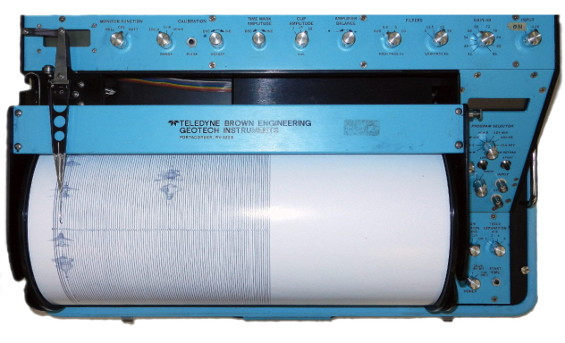
\includegraphics[scale=0.35]{registrador.png}
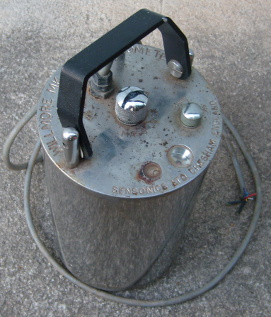
\includegraphics[scale=0.35]{sensor.png}
\caption{Registrador Teledyne modelo Portacorder (esquerda) e sensor
  Willmore MKII (direita) utilizados em diversas estações operadas
  pelo IAG/USP de 1976 à 1995. O registrador é capaz de filtrar o
  sinal emitido pelo sensor por um sistema de filtros passa-banda e
  registra-lo em papel. O tempo de registro por folha podia ser
  regulado de 1.9 horas a 120 horas. O relógio do equipamento era
  aferido utilizando-se rádios relógio mundiais como a WWV no
  Colorado/US que era então super-imposto nos registros em intervalos
  ajustáveis de hora, minuto, 1 segundo ou 10 segundos.}
\label{teledyne}
\end{center}
\end{figure}
Os registros em papel (Figura~\ref{sismograma}) eram analisados um a um com o auxílio
de lupas, réguas de leitura e de conversão de centímetros em amplitude
de vibração do solo. Marcações de tempo eram interpretadas para aferir
o relógio do instrumento, garantindo assim uma precisão de décimos a
centésimos de segundo. Os tempos de chegadas das ondas sísmicas (fases
P, S ou de Superfície) emitidas por terremotos registradas pelas
estações eram então determinados. Com os tempos de chegada em mais de
uma estação determinavam-se Epicentros de tremores, que eram então
investigados buscando determinar as suas causas e compunham então o
Boletim Sísmico Brasileiro (BSB) e mesmo, em 1982 permitiram o
IAG/USP, em parceria com outras instituições do Brasil confeccionar o
livro Sismicidade do Brasil, ganhador do prêmio Jabuti de 1985 na área
de Ciências Exatas~\cite{sismicidade-brasil}.

Parte do projeto de digitalização deste acervo visa permitir novamente
que sismólogos de todo o Brasil e mesmo de outras instituições
mundiais tenham novamente acesso aos dados, sendo capazes de
reanalisar os registros e mesmo, validar pesquisas anteriormente
feitas. Neste processo, é necessário além de digitalizar os registros
(tarefa que esta sendo feita por alunos no IAG/USP) desenvolver
metodologias e ferramentas de análise.
\begin{figure}[htb]
  \begin{center}
    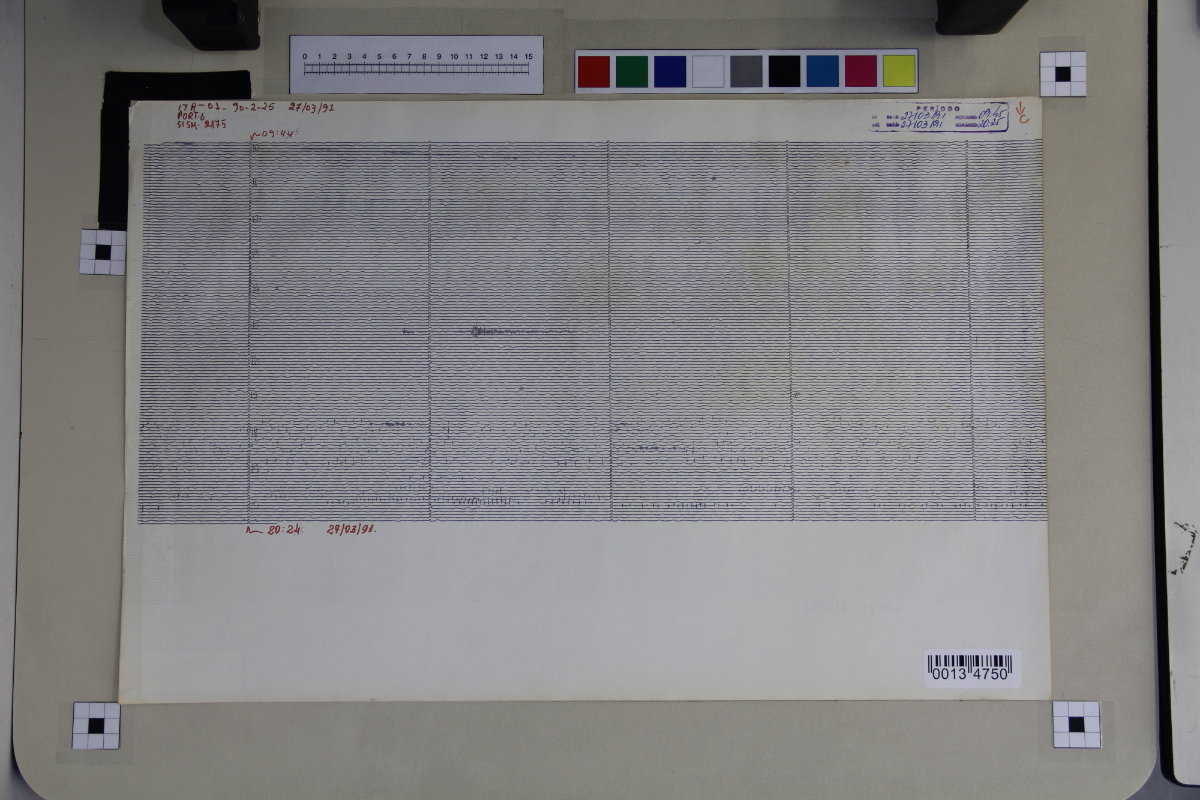
\includegraphics[scale=0.25]{sismograma.jpg}
\caption{Sismograma teste digitalizado. O registro em questões foi
  feito pela estação ITR em 1991. Cada sismograma é identificado por
  um código de barras (canto direito inferior), normalmente contém
  metadados na parte superior e pode ter sido já interpretado (marcas
  a lápis sobre o registro). No registro em questões podemos observar
  as ondas proveniente de um abalo provavelmente regional
  aproximadamente no centro do registro (área com maior “densidade” de
  tinta no centro-esquerdo da folha).}
\label{sismograma}
\end{center}
\end{figure}
O processo de disponibilizar os sismogramas carece do desenvolvimento
de técnicas especificas para permitir o processamento das imagens como
se fossem registros em papel, implicando assim em: (a) Estabelecer na
imagem um sistema de referência permitindo ao usuário realizar
leituras de tempo e amplitude da onda e (b) Permitir que o usuário
realize anotação em determinadas posições da imagem. Ambas
informações devem de certa forma ser associadas a cada imagem e
tecnologias como cabeçalhos EXIF~\cite{exif} ou mesmo encapsulamento
SVG~\cite{svg}, que devem ser estudadas para serem estendidas tentando
suprir assim as necessidades do projeto. 





O processo de estabelecer o sistema de referência na imagem pode ser
auxiliado pela utilização de algoritmos simples de processamento e
reconhecimento de padrões especialmente designados para este fim. As
marcas de tempo por exemplo (Figura~\ref{detalhe}) podem ser extraídas pela
correlação cruzadas de uma amostra do padrão de tempo com a própria
imagem, auxiliando assim o usuário a criar o sistema de referência de
tempo. O sistema de referência da escala de amplitude deve ser feito
utilizando referências externas (marcas de controle na foto não
pertencentes ao sinal) para converter pixels em cm na foto) e utilizar
assim agora os parâmetros de ganho (disponíveis nos metadados da
imagem) para converter de cm para amplitude de vibração do solo.

Capacidades de mark-up a serem desenvolvidas podem inicialmente
habilitar a anotação da imagem com marcas de texto livre, e marcas de
localização hipocentrais e leituras de fases. As marcas de localização
hipocentrais devem implementar as seguintes propriedades: Longitude,
Latitude, Profundidade, Hora de Origem e  Magnitude. As leituras de
fases, que podem ou não serem associadas a localizações hipocentrais
devem implementar as seguintes propriedades: Tempo, Amplitude e Tipo
(fase P, S e Superficial).

\begin{figure}
  \begin{center}
    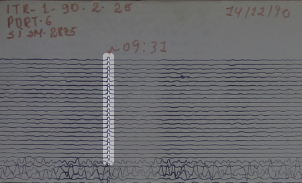
\includegraphics[scale=1.1]{detalhe.png}
    \caption{Detalhe do sismograma apresentado na Figura~\ref{sismograma} mostrando as marcações
      de tempo feitas pelo Portacorder. As marcações de tempo eram
      superimpostas no sinal pelo instrumento e tem um formato retangular
      onde a sua largura indica o tipo de marca. A marca destacada
      corresponde aos tempos de minuto cheio. Tais marcas podem facilmente
      serem automaticamente identificadas por algorítimos de
      auto-correlação de uma amostra do sinal extraído da própria imagem
      com ela mesma.}
    \label{detalhe}
  \end{center}
\end{figure}

Ao final, o processo de migrar o formato os dados analógicos dos
sismogramas em papel requer a aplicação de tecnologias existentes de
forma a permitir ao usuário que o dado volte a ser utilizado ao seu
máximo. Esses dados históricos cobrem um período histórico importante
da sismicidade brasileira. Eles são os dados brutos de diversos
estudos realizados no Brasil e caso sejam perdidos ou, não seja mais
possível analisá-los não será mais possível validar novas pesquisas
sendo desenvolvidas utilizado o BSB, como por exemplo análises de
risco sísmico e mesmo estudos de sismicidade que buscam compreender
como que esforços tectônicos interagem com a placa Sul Americana,
gerando assim o padrão e sismicidade observado no Brasil nos últimos
35 anos (Figura~\ref{sismicidade}).


\begin{figure}[htb]
  \begin{center}
    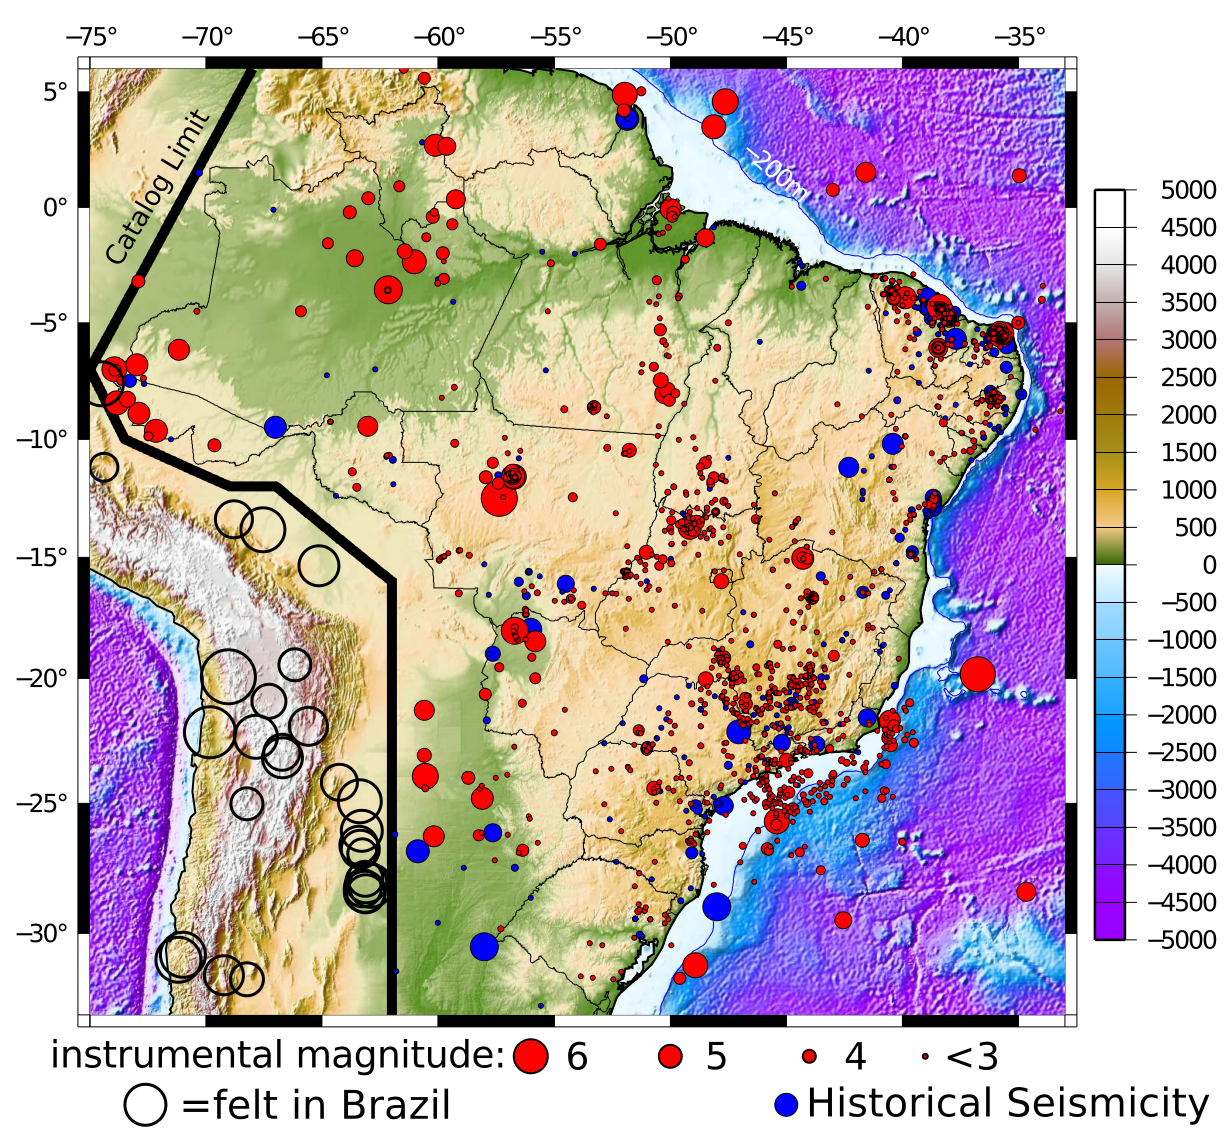
\includegraphics[scale=0.4]{mapa.png}
    \caption{Sismicidade brasileira de 1720-2015/02 como reportado
      pelo BSB preparado pelo centro de sismologia da Universidade de
      São Paulo. Cada círculo no mapa indica um sismo catalogado pelo
      BSB. Os sismos históricos (círculos em azul) são sismos determinados por pesquisas
      macro-sísmicas enquanto que sismos em vermelho são sismos
      determinados instrumentalmente, via registros em papel ou em
      forma digital a partir de 1992-1995. O tamanho do círculo indica
      da magnitude do evento na escala Richter de magnitudes.}
    \label{sismicidade}
  \end{center}
\end{figure}




\section{Objetivos e metas}

O objetivo científico do projeto é contribuir para a preservação do
registro histórico dos sismogramas e magnetogramas, além de
dar um passo inicial para a futura análise desses dados, na forma de
software voltado para a representação e visualização deles.

Para a formação da aluna, o objetivo é exatamente o do programa PDPD;
especificamente, esperamos que a aluna tome contato com a pesquisa
em geofísica, através de sua inserção em um projeto {\em real} e
{\em relevante}, e que desenvolva a capacidade de estudo e elaboração
autônoma de soluções em computação aplicada.

As metas são:
\begin{itemize}
\item[i) ] {\bf especificar} uma estrutura para representar metadados de anotações feitas em imagens digitalizadas
  de sismogramas e magnetogramas;
\item[ii) ] implementar uma {\bf biblioteca} para incluir e recuperar os
  dados na estrutura definida;
\item[iii) ] implementar {\em um} {\bf algoritmo} para tentar identificar
  automaticamente alguma característica das imagens que seja
  interessante do ponto de vista da geofísica;
\item[iv) ] implementar {\bf interface} de visualização para {\em parte}
  dos metadados, usando a biblioteca.
\end{itemize}

Não há compromisso em obter resultados de alta precisão no desempenho
do algoritmo mencionado ma meta (iii), dado que a aluna é ingressante
no BC\&T -- o objetivo desta meta é principalmente o de familiarizar
a aluna com o trabalho de pesquisa na área.
A meta (iv) poderá ser implementada de maneira simplificada, e para
apenas parte das anotações (possivelmente só um campo).

Todo o software produzido será disponibilizado com licença livre.

\section{Metodologia de trabalho}

Este trabalho é essencialmente exploratório, consituindo pesquisa
aplicada de Computação em Sismologia. A aluna deverá realizar revisão
bibliográfica básica sobre representação de metadados em imagens e
em reconhecimento de padrões (de maneira limitada e direcionada pelo
orientador), seguida de implementações.

Especificamente, a aluna estudará modos de encapsulamento de metadados
em imagens, a fim de definir o padrão para markup; implementará um
protótipo simples desse padrão; estudará alguns algoritmos simples
para processamento de imagens~\cite{gonzalez,burger}; e implementará um
destes algoritmos.


\section{Cronograma}

A tabela a seguir mostra o cronograma de atividades para a aluna. Além
das metas já descritas, há duas atividades de revisão bibliográfica: a
primeira com o foco em estruturas para armazenamento de metadados de
imagens, e a segunda com o foco em algoritmos para processamento de
imagens.

\begin{center}
\scalebox{0.85}{
\begin{gantt}[fontsize=\small,titlefontsize=\small]{7}{10}
\begin{ganttitle}
  \numtitle{1}{1}{10}{1}
\end{ganttitle}
\ganttbar[pattern=none,fill=blue!40]{revisão biblio}{0}{1}
\ganttbar[pattern=none,fill=blue!40]{especificação}{1}{1}
\ganttbar[pattern=none,fill=blue!40]{biblioteca}{2}{2}
\ganttbar[pattern=none,fill=blue!40]{revisão biblio}{4}{3}
\ganttbar[pattern=none,fill=blue!40]{algoritmo}{5}{3}
\ganttbar[pattern=none,fill=blue!40]{interface}{8}{2}
\end{gantt}
}
\end{center}


\section{Adequação do projeto à aluna}

Salientamos que, embora ingressante na UFABC, a aluna já sabe
programar e tem prática em desenvolvimento Web. Além disso,
não pretendemos que seja necessário utilizar quaisquer técnicas difícies
de processamento de imagens (a aluna poderá, por exemplo, usar apenas
técnicas básicas no domínio espacial).

\printbibliography

\blfootnote{Texto e figuras produzidos integralmente em \LaTeX, exceto
  fotos.}

\end{document}

